\appendix
\section{Additional results of post-processing a single NWP forecasting model}
\label{appendix:single}

\paragraph{MAE}
\begin{figure}[htb!]
    \centering
    \begin{subfigure}{\columnwidth}
        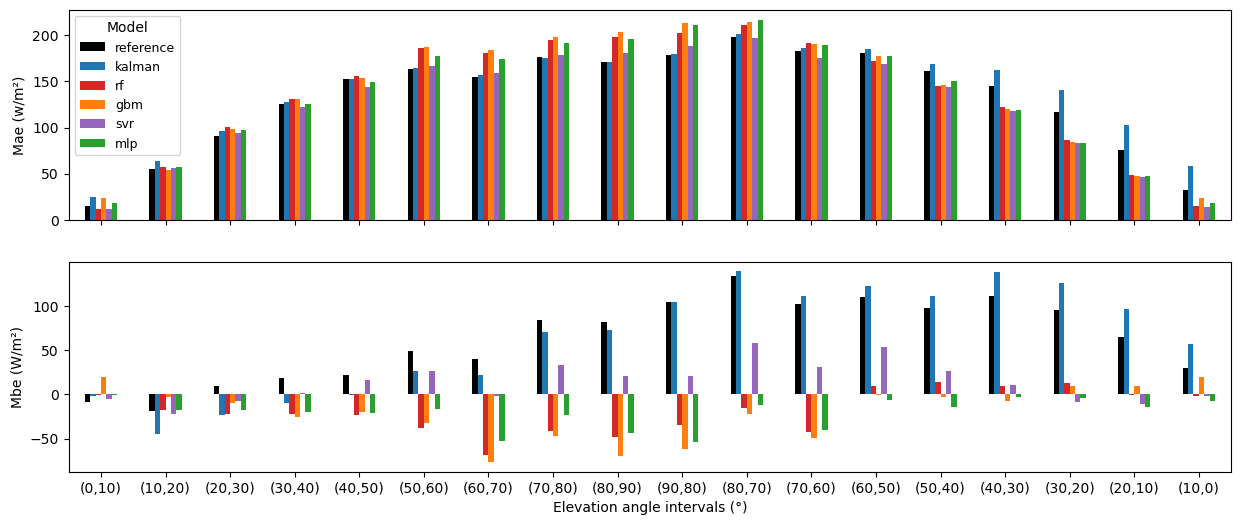
\includegraphics[width=\columnwidth]{figures/first_study/mae_mbe_site1.png}
        \subcaption{Site 1}
    \end{subfigure}
\medskip
    \begin{subfigure}{\columnwidth}
        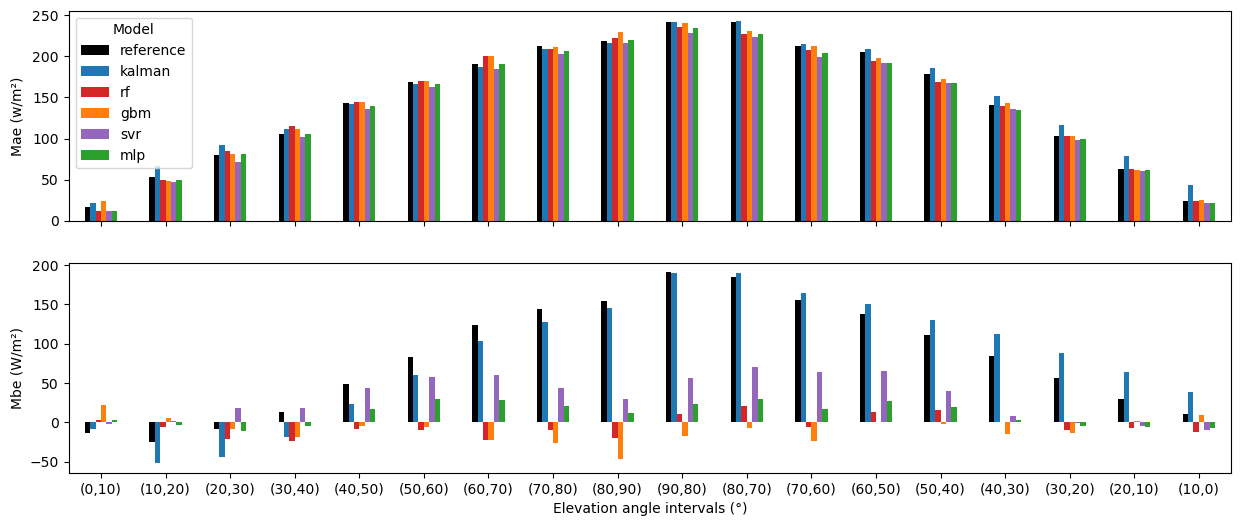
\includegraphics[width=\columnwidth]{figures/first_study/mae_mbe_site3.png}
        \subcaption{Site 3}
    \end{subfigure}
\medskip
    \begin{subfigure}{\columnwidth}
        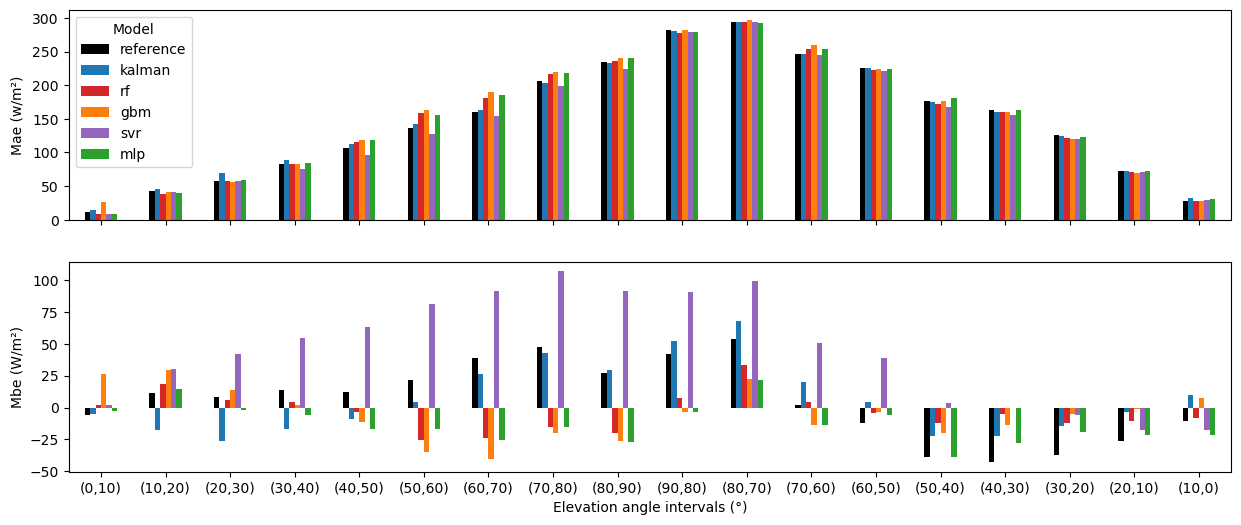
\includegraphics[width=\columnwidth]{figures/first_study/mae_mbe_site4.png}
        \subcaption{Site 4}
    \end{subfigure}
    \caption[]{MAE and MBE levels across all elevation angle intervals of a day.}
\end{figure}

\begin{figure}[htb!]
    \centering
    \begin{subfigure}{\columnwidth}
        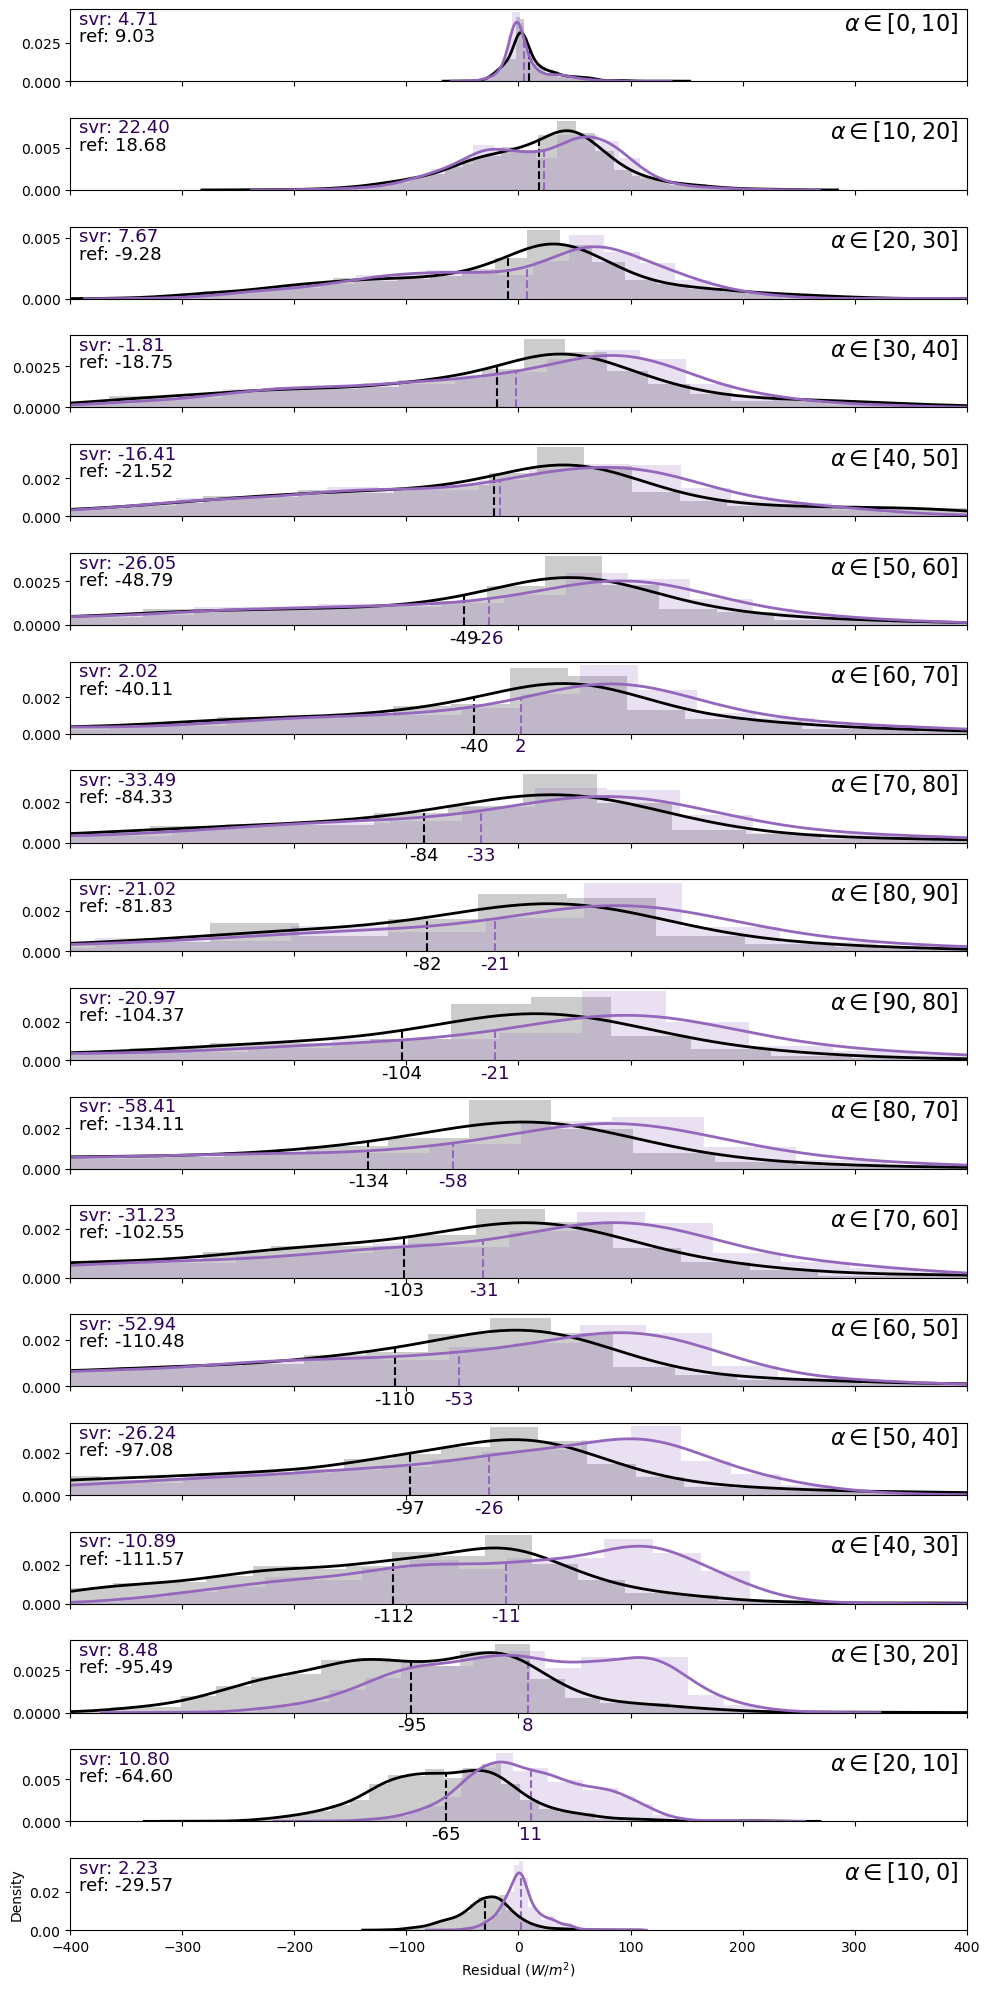
\includegraphics[width=\columnwidth]{figures/first_study/residual_errors_svr_site1_mae.png}
        \subcaption{Site 1}
    \end{subfigure}
\medskip
    \begin{subfigure}{\columnwidth}
        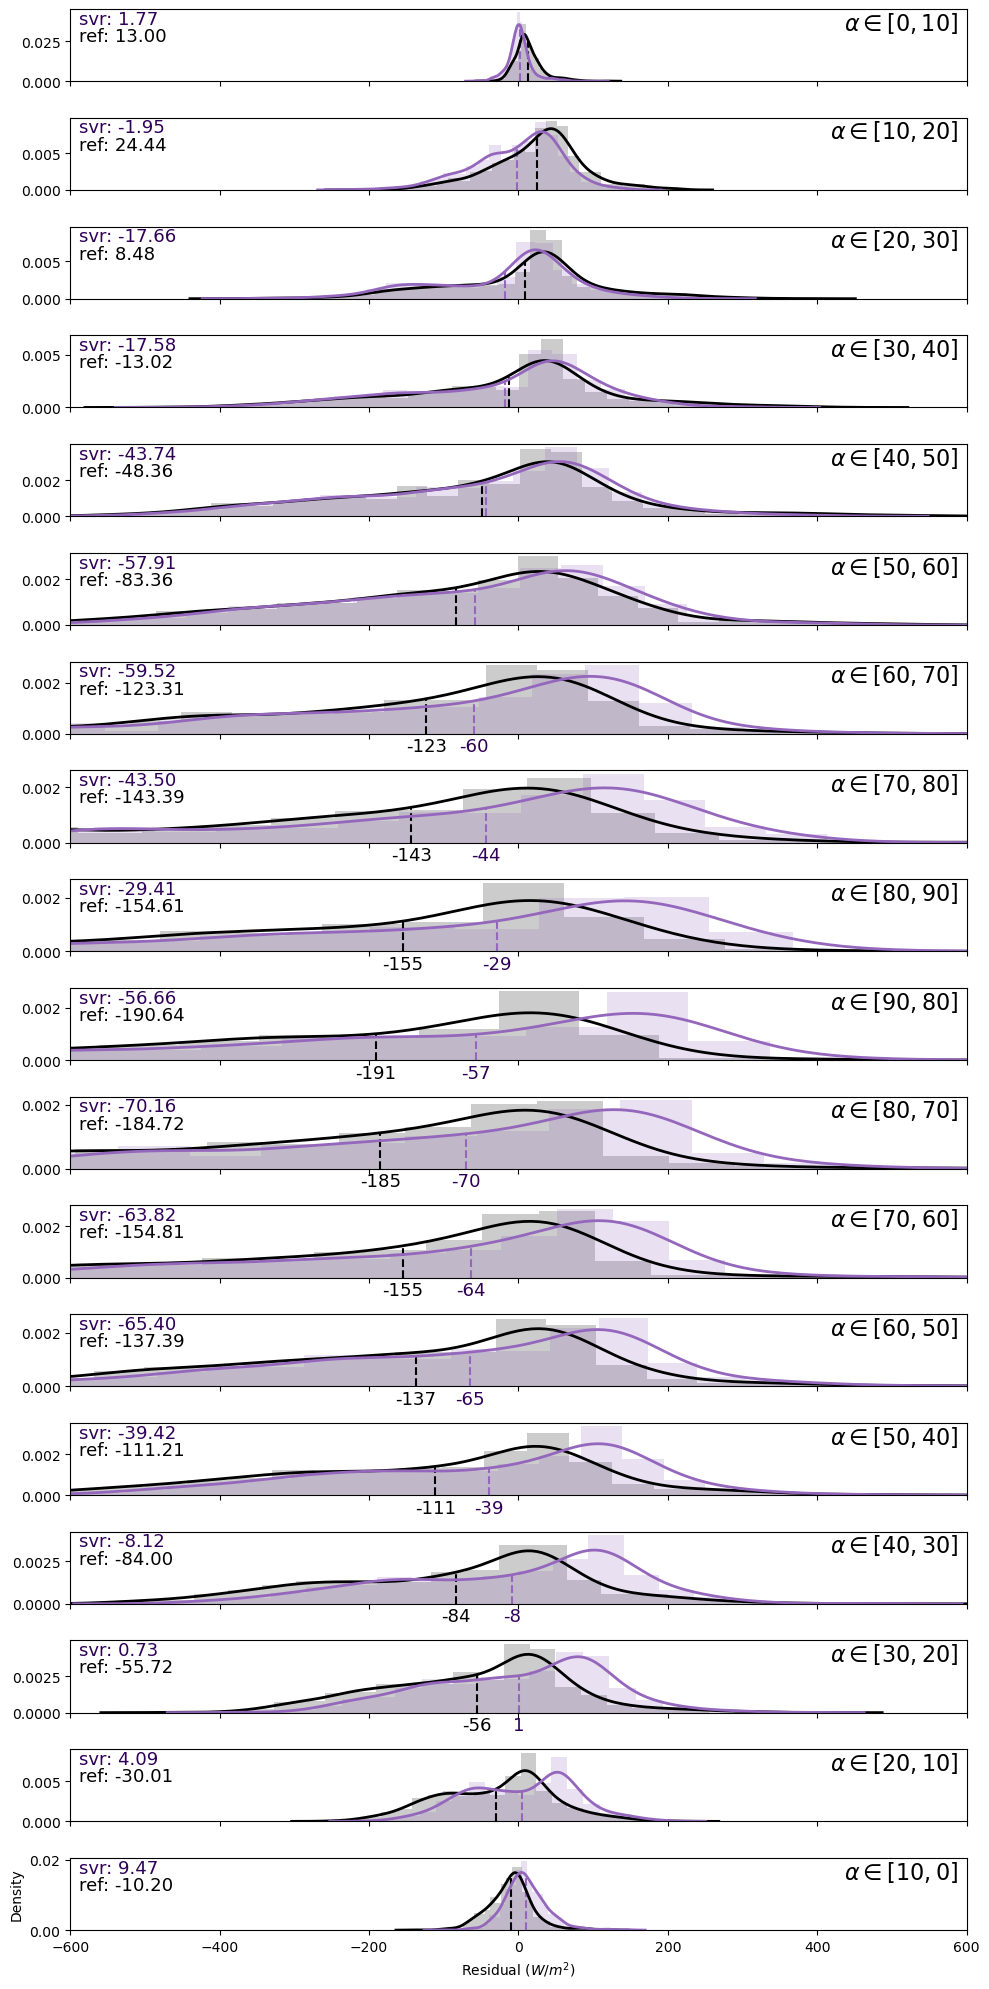
\includegraphics[width=\columnwidth]{figures/first_study/residual_errors_svr_site3_mae.png}
        \subcaption{Site 3}
    \end{subfigure}
\medskip
    \begin{subfigure}{\columnwidth}
        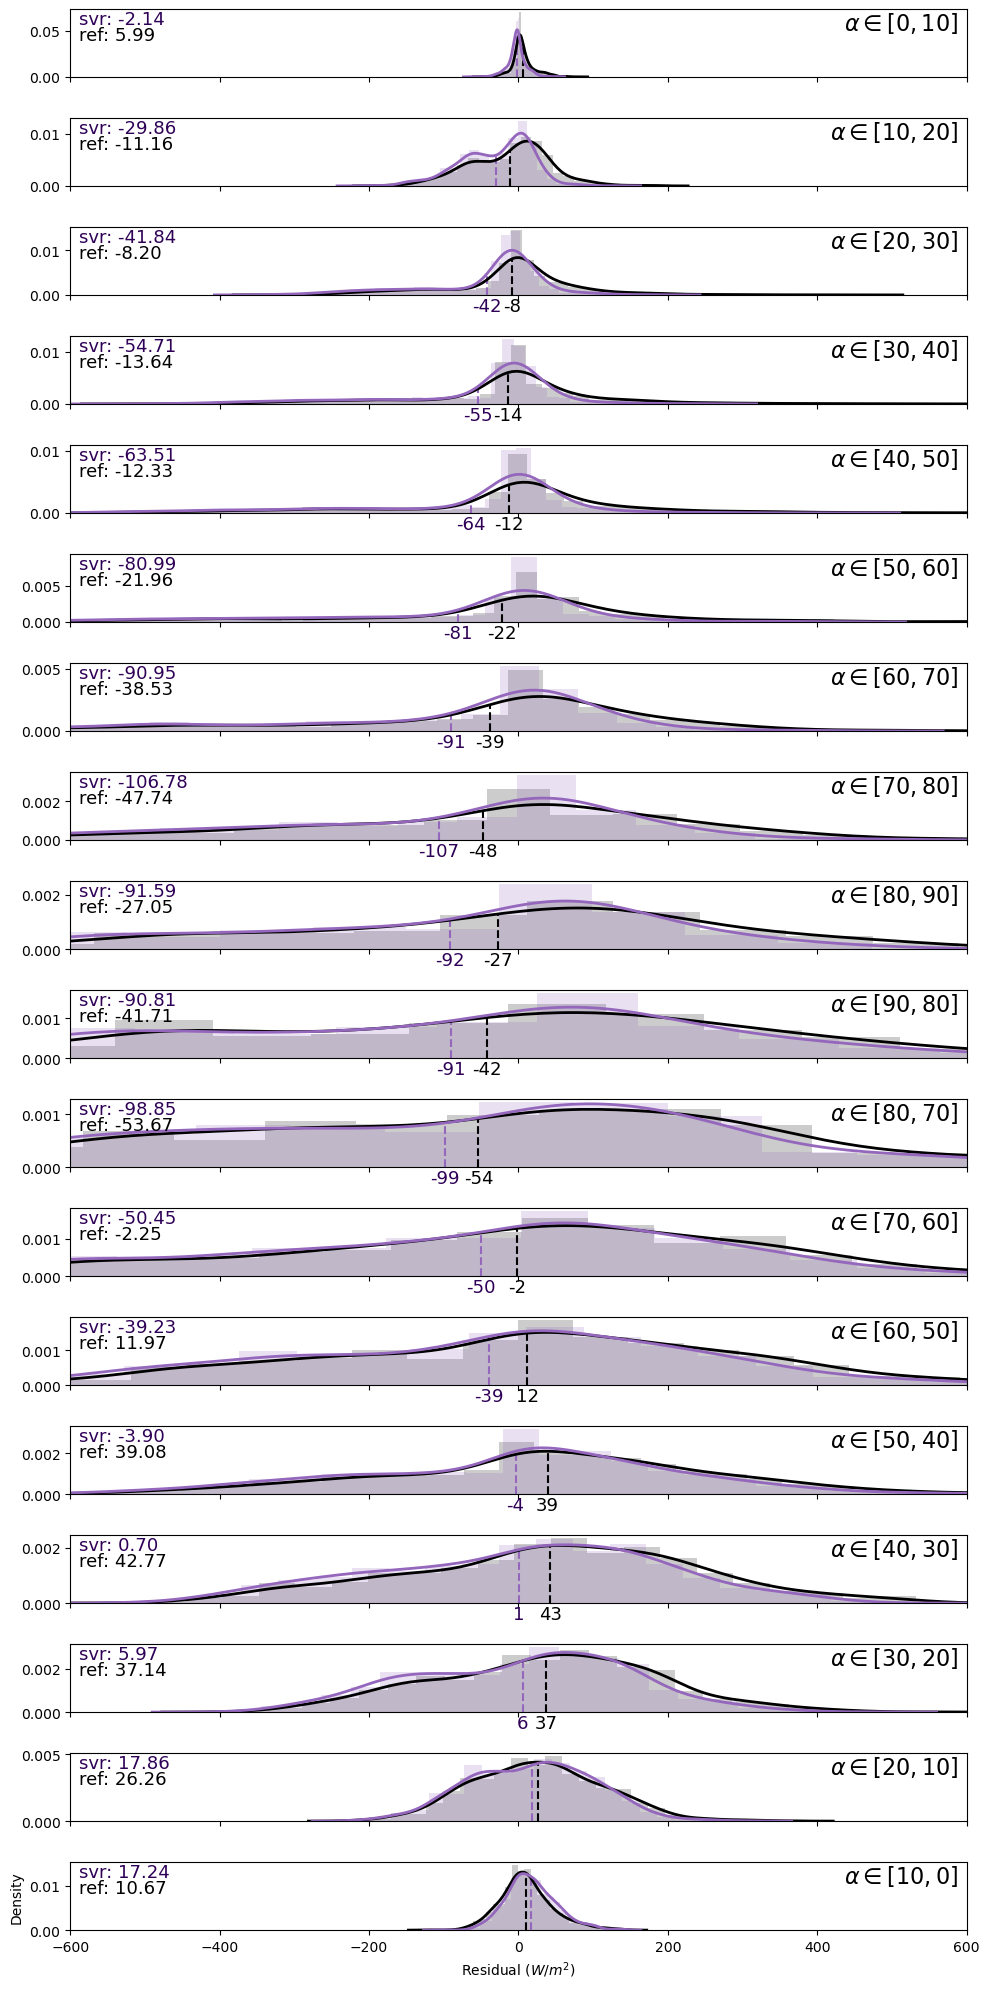
\includegraphics[width=\columnwidth]{figures/first_study/residual_errors_svr_site4_mae.png}
        \subcaption{Site 4}
    \end{subfigure}
    \caption[]{Residual error levels across all elevation angle intervals of a day, for a SVR model.}
\end{figure}


\begin{figure}[htb!]
    \centering
    \begin{subfigure}{\columnwidth}
        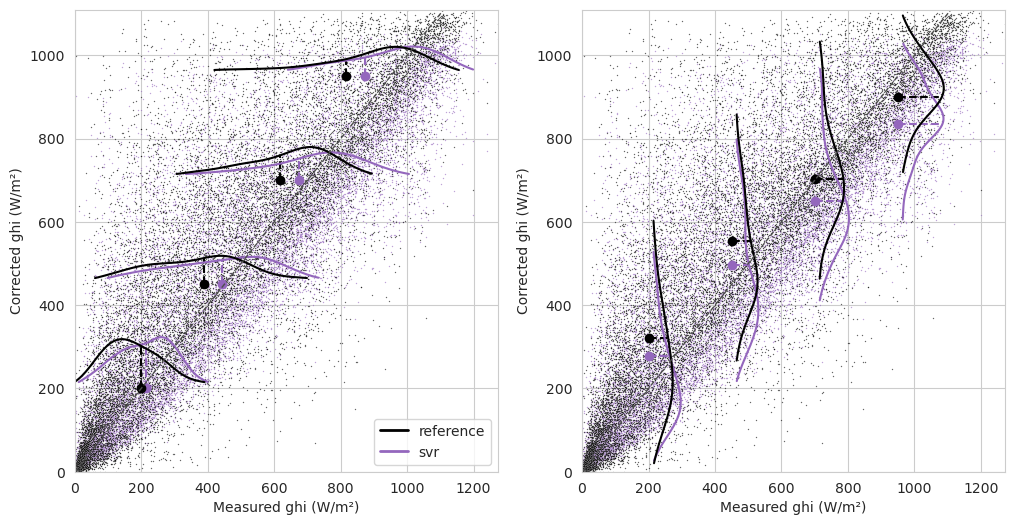
\includegraphics[width=\columnwidth]{figures/first_study/scatter_plot_svr_site1_mae.png}
        \subcaption{Site 1}
    \end{subfigure}
\medskip
    \begin{subfigure}{\columnwidth}
        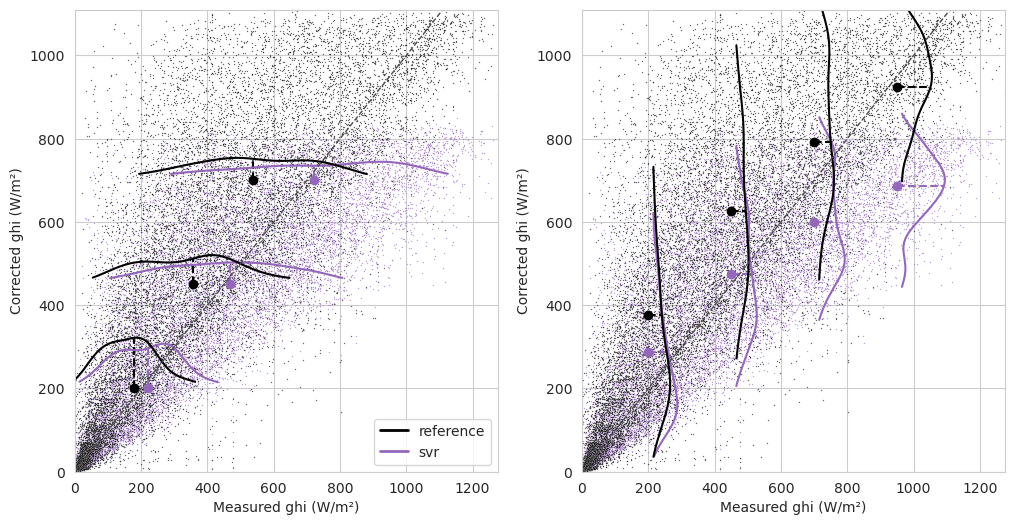
\includegraphics[width=\columnwidth]{figures/first_study/scatter_plot_svr_site2_mae.png}
        \subcaption{Site 2}
    \end{subfigure}
\medskip

    \begin{subfigure}{\columnwidth}
        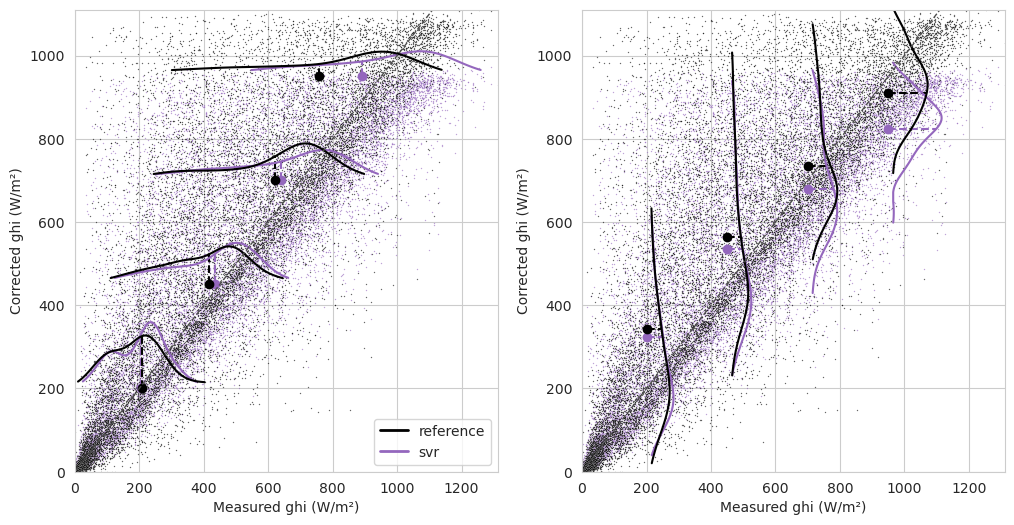
\includegraphics[width=\columnwidth]{figures/first_study/scatter_plot_svr_site3_mae.png}
        \subcaption{Site 3}
    \end{subfigure}
\medskip
    \begin{subfigure}{\columnwidth}
        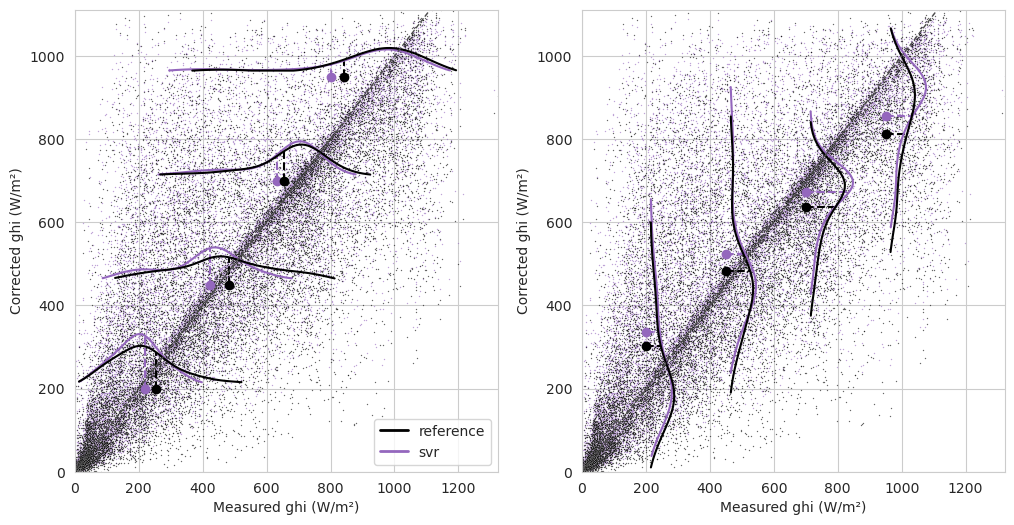
\includegraphics[width=\columnwidth]{figures/first_study/scatter_plot_svr_site4_mae.png}
        \subcaption{Site 4}
    \end{subfigure}
    \caption[]{Scatter plots for a SVR model against the reference model.}
\end{figure}
\paragraph{RMSE}
\begin{figure}[htb!]
    \centering
    \begin{subfigure}{\columnwidth}
        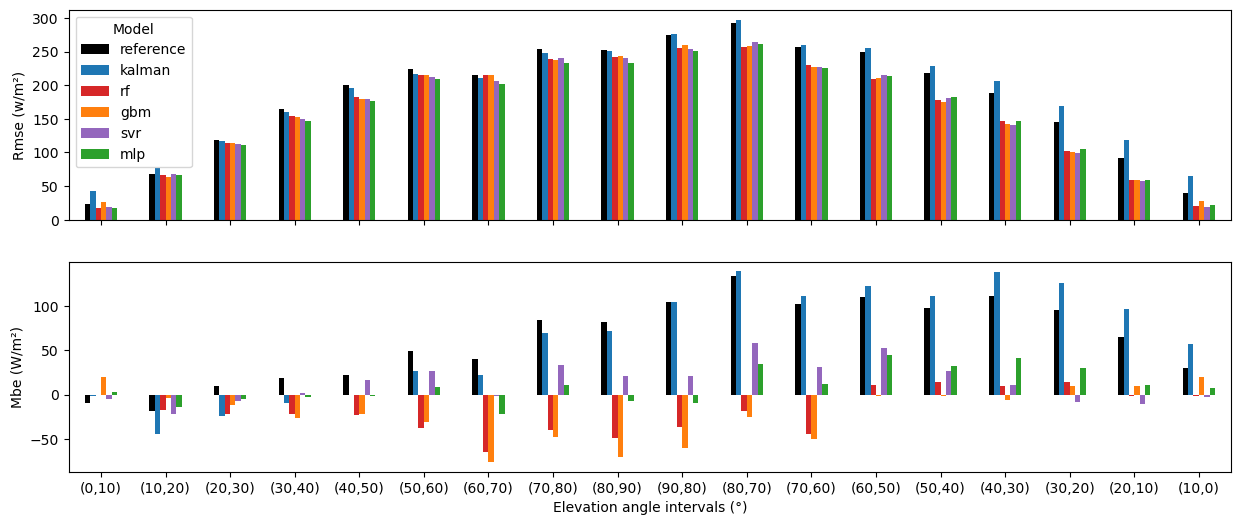
\includegraphics[width=\columnwidth]{figures/first_study/rmse_mbe_site1.png}
        \subcaption{Site 1}
    \end{subfigure}
\medskip
    \begin{subfigure}{\columnwidth}
        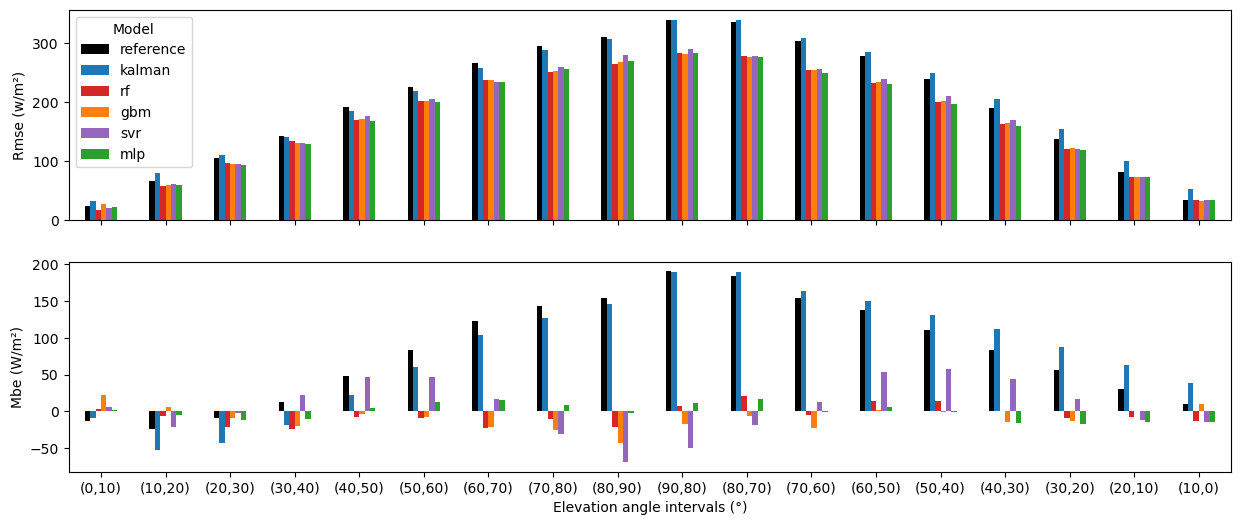
\includegraphics[width=\columnwidth]{figures/first_study/rmse_mbe_site3.png}
        \subcaption{Site 3}
    \end{subfigure}
\medskip
    \begin{subfigure}{\columnwidth}
        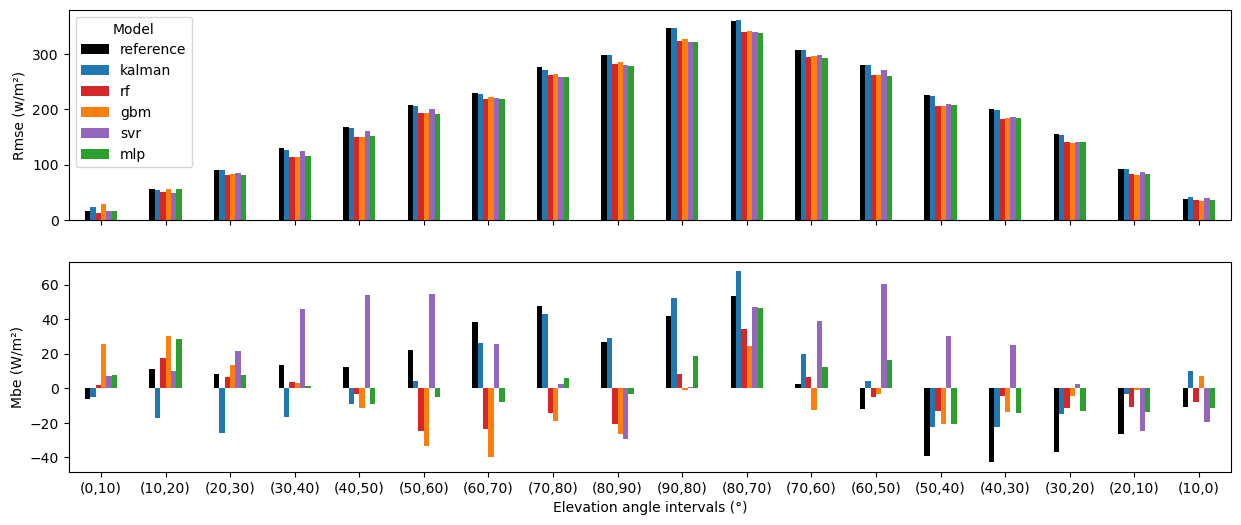
\includegraphics[width=\columnwidth]{figures/first_study/rmse_mbe_site4.png}
        \subcaption{Site 4}
    \end{subfigure}
    \caption[]{RMSE and MBE levels across all elevation angle intervals of a day.}
\end{figure}


\begin{figure}[htb!]
    \centering
    \begin{subfigure}{\columnwidth}
        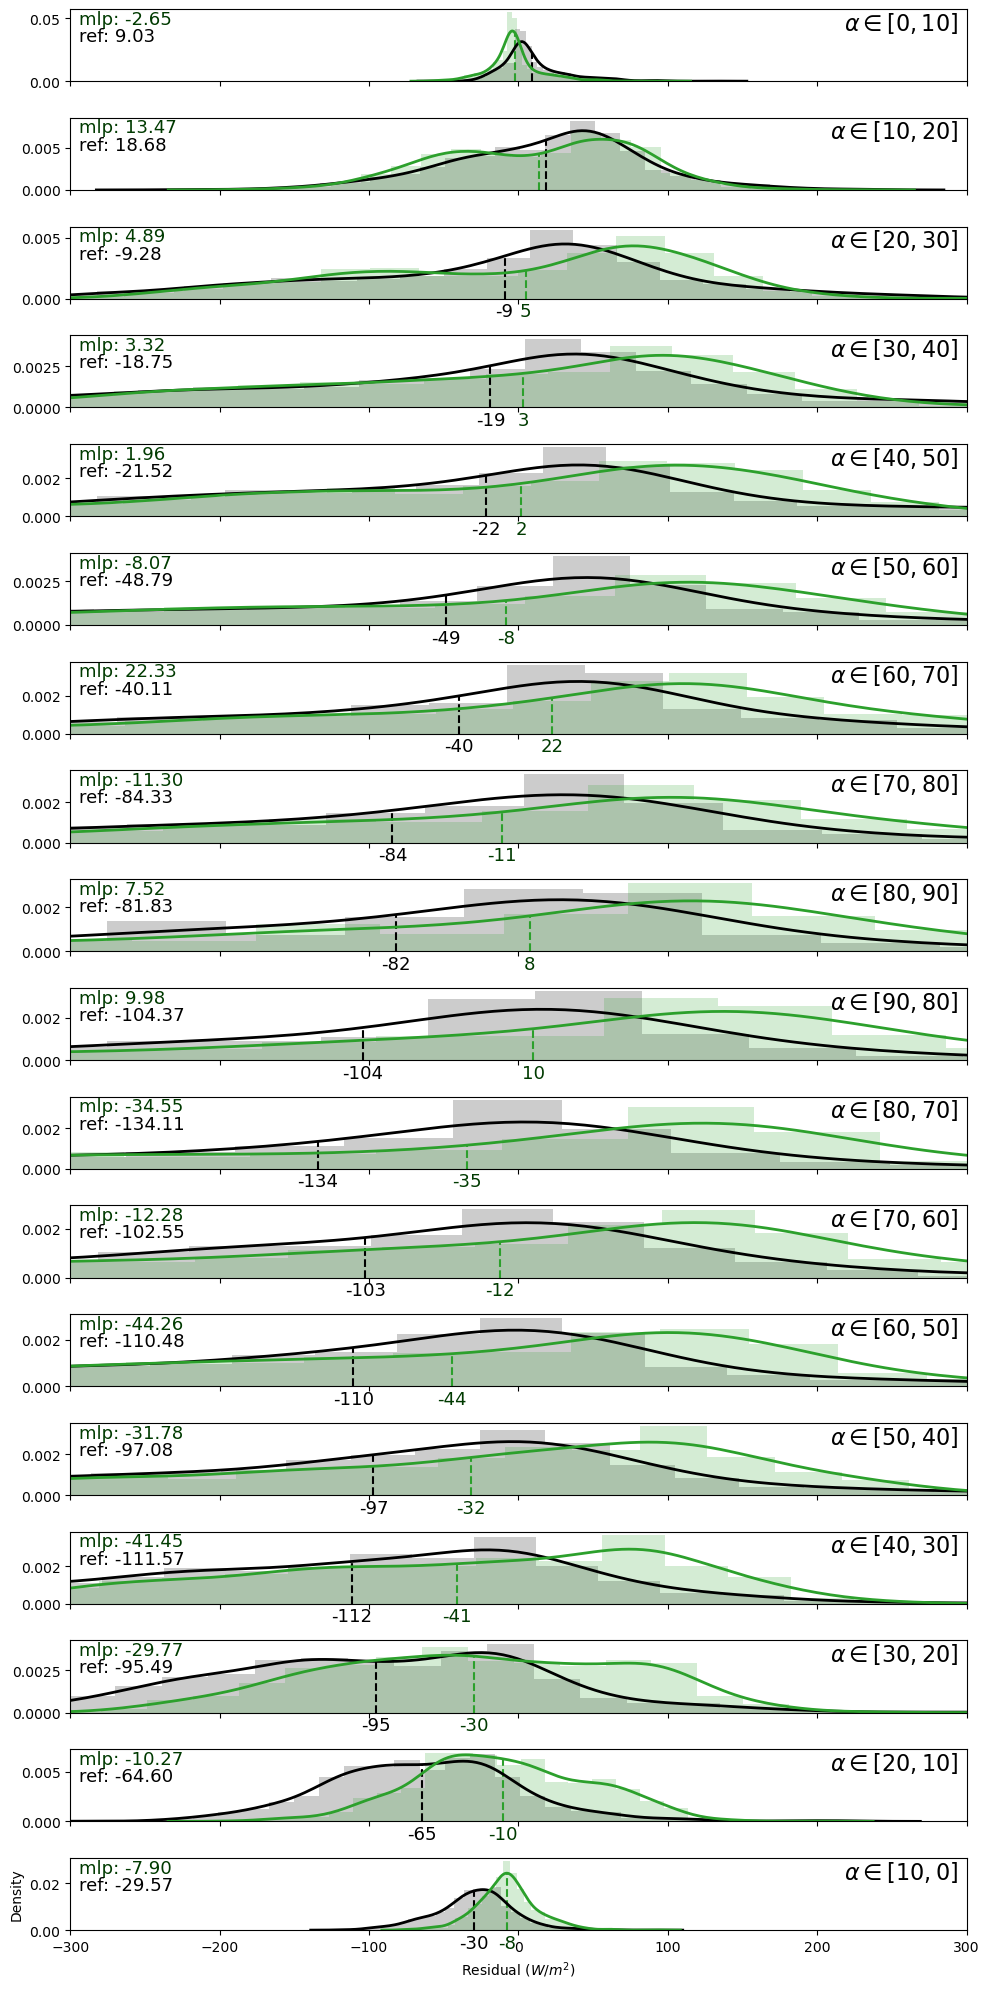
\includegraphics[width=\columnwidth]{figures/first_study/residual_errors_mlp_site1_rmse.png}
        \subcaption{Site 1}
    \end{subfigure}
\medskip
    \begin{subfigure}{\columnwidth}
        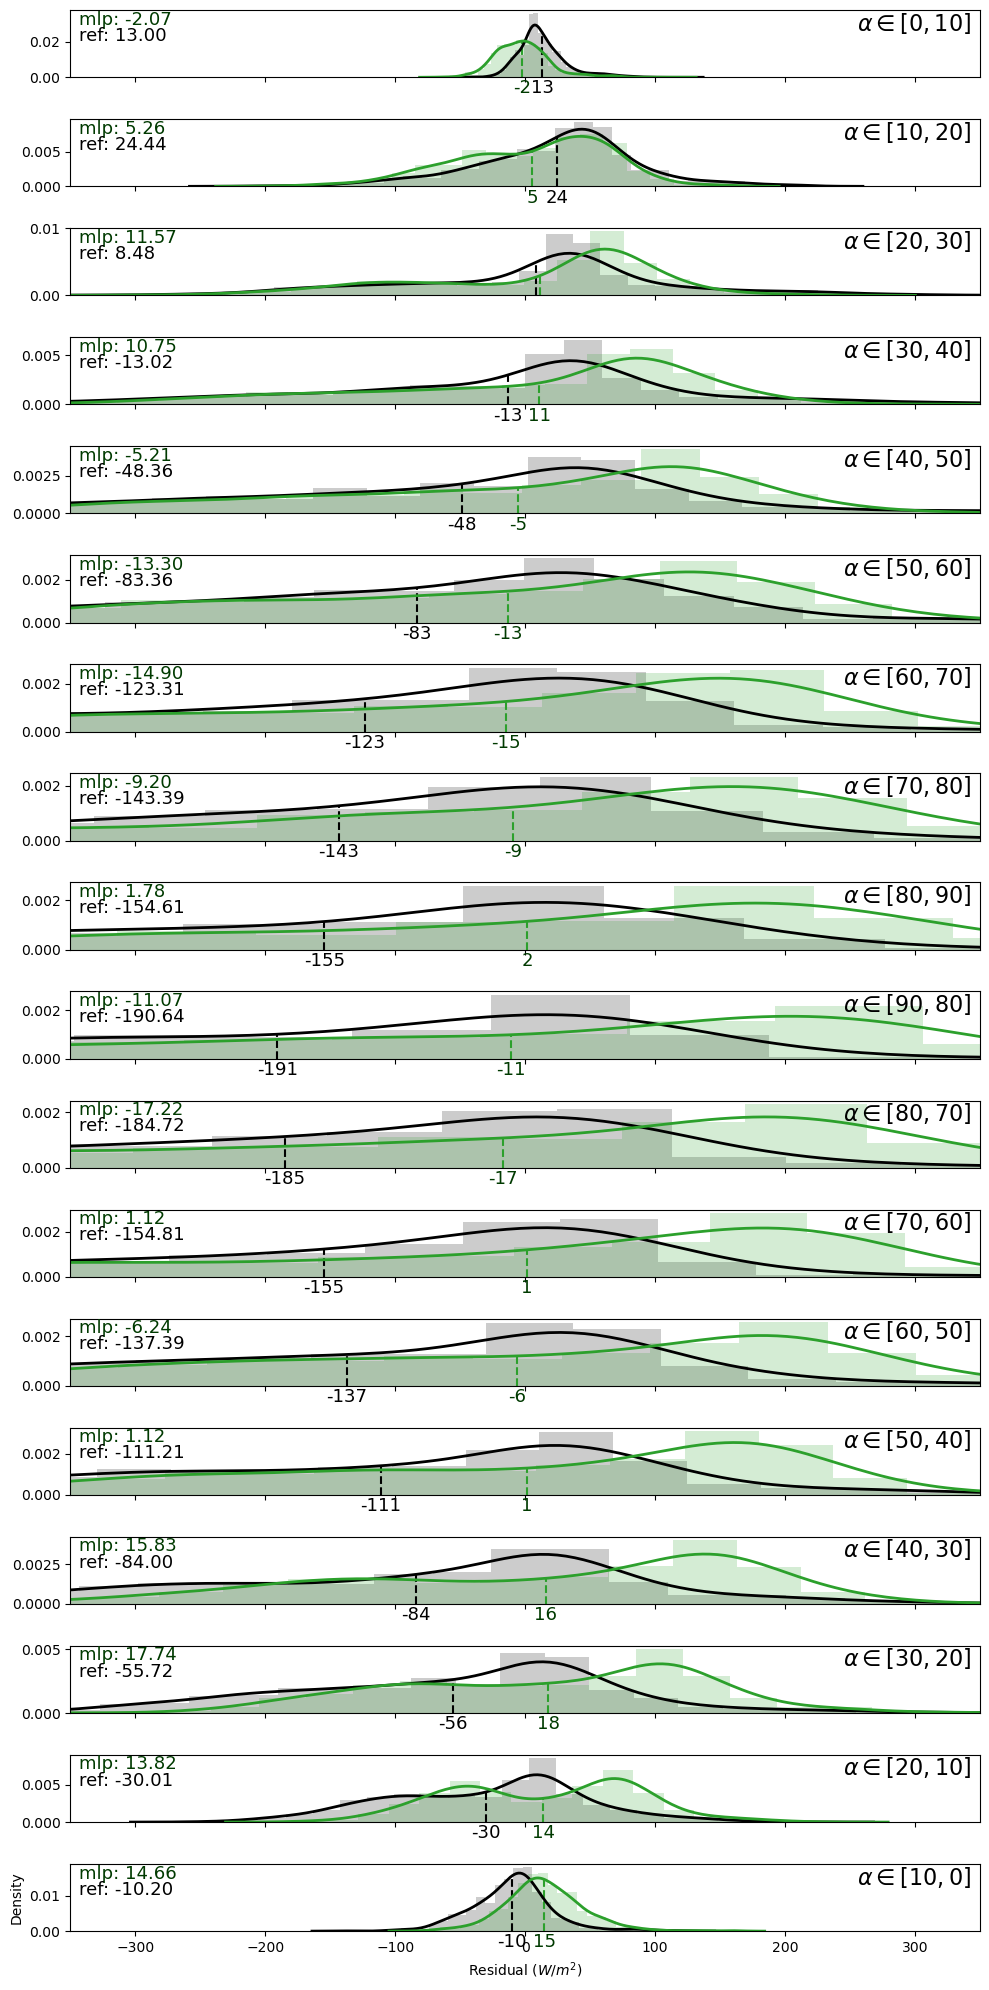
\includegraphics[width=\columnwidth]{figures/first_study/residual_errors_mlp_site3_rmse.png}
        \subcaption{Site 3}
    \end{subfigure}
\medskip
    \begin{subfigure}{\columnwidth}
        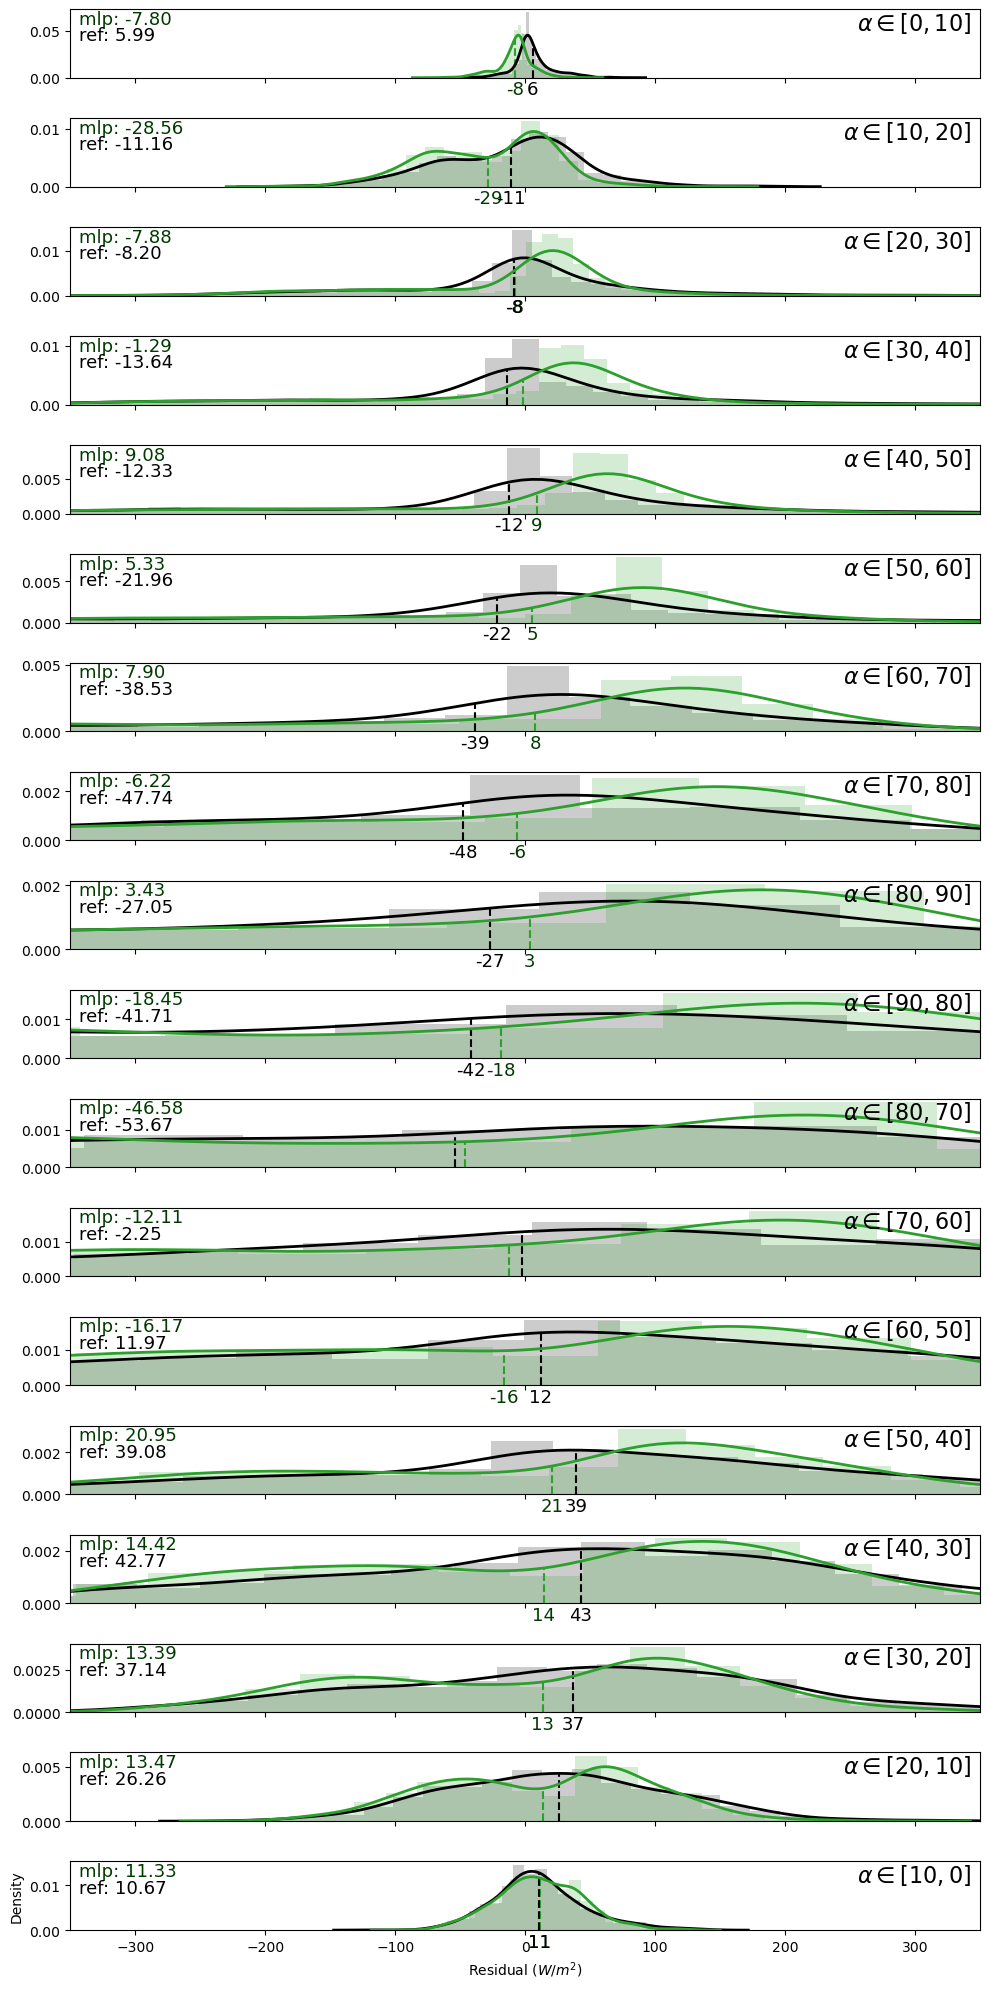
\includegraphics[width=\columnwidth]{figures/first_study/residual_errors_mlp_site4_rmse.png}
        \subcaption{Site 4}
    \end{subfigure}
    \caption[]{Residual error levels across all elevation angle intervals of a day, for a MLP model.}
\end{figure}


\begin{figure}[htb!]
    \centering
    \begin{subfigure}{\columnwidth}
        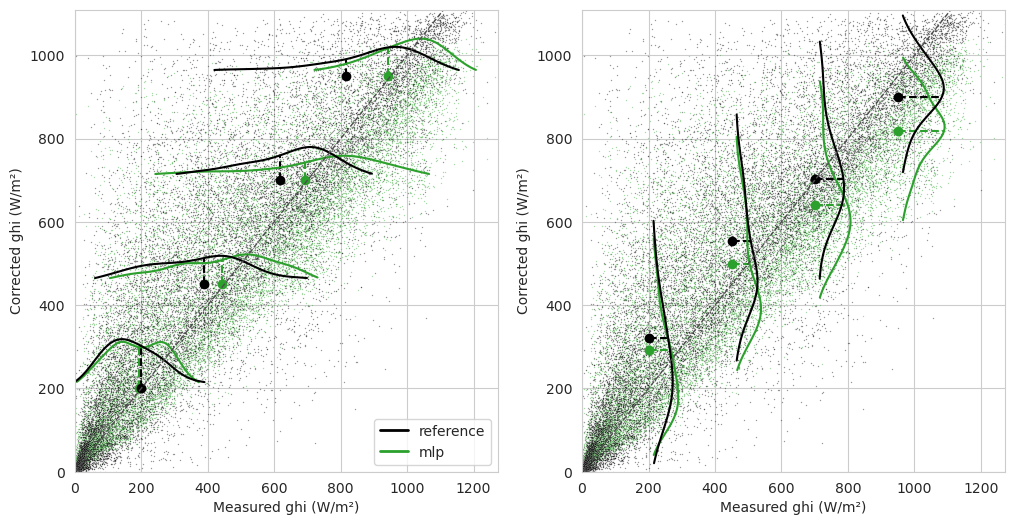
\includegraphics[width=\columnwidth]{figures/first_study/scatter_plot_mlp_site1_rmse.png}
        \subcaption{Site 1}
    \end{subfigure}
\medskip
    \begin{subfigure}{\columnwidth}
        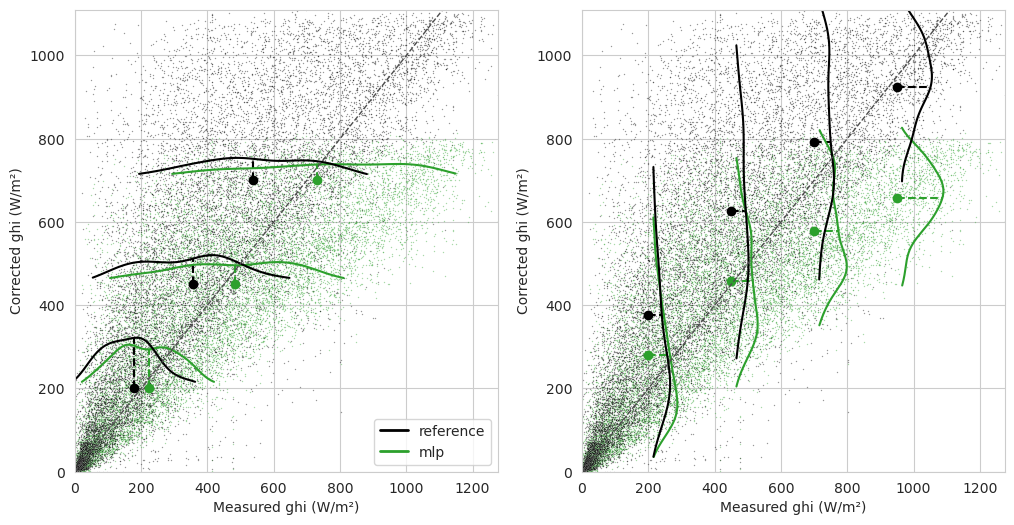
\includegraphics[width=\columnwidth]{figures/first_study/scatter_plot_mlp_site2_rmse.png}
        \subcaption{Site 2}
    \end{subfigure}
\medskip

    \begin{subfigure}{\columnwidth}
        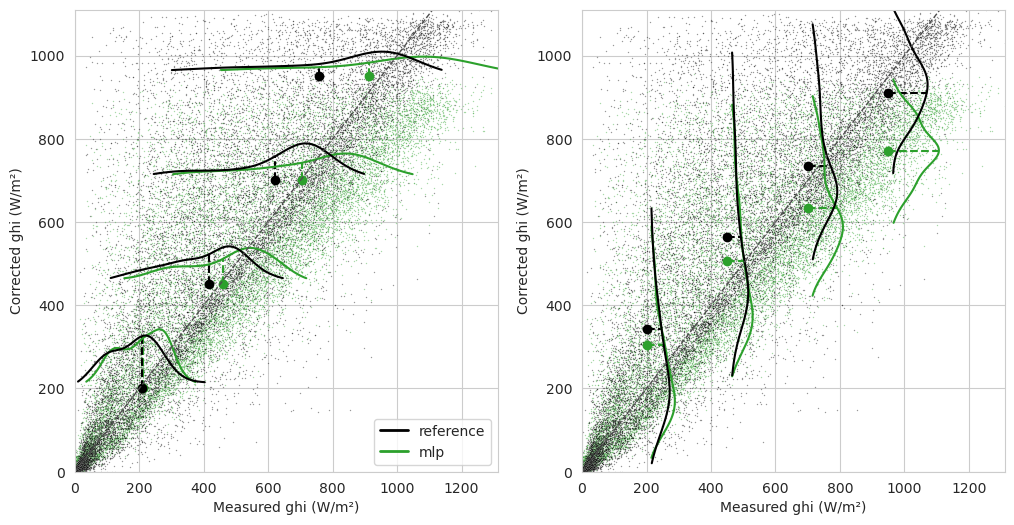
\includegraphics[width=\columnwidth]{figures/first_study/scatter_plot_mlp_site3_rmse.png}
        \subcaption{Site 3}
    \end{subfigure}
\medskip
    \begin{subfigure}{\columnwidth}
        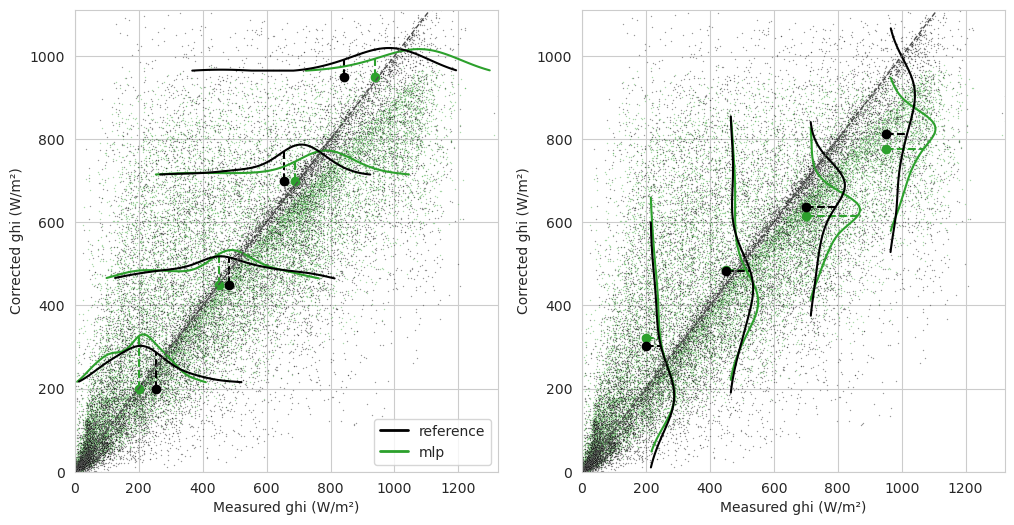
\includegraphics[width=\columnwidth]{figures/first_study/scatter_plot_mlp_site4_rmse.png}
        \subcaption{Site 4}
    \end{subfigure}
    \caption[]{Scatter plots for a MLP model against the reference model.}
\end{figure}


\begin{figure}[htb!]
    \centering
    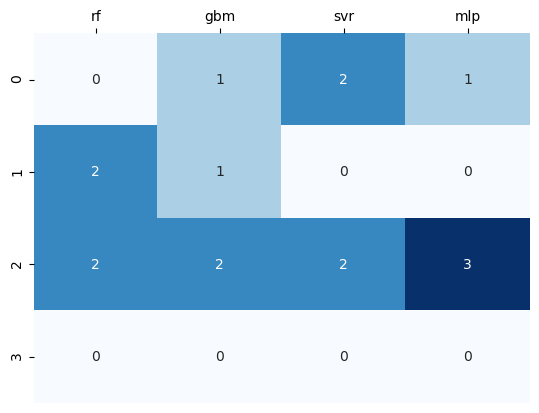
\includegraphics[width=\columnwidth]{figures/first_study/comp_predictors_rmse.png}
\caption{Pairwise systematicity matrix for RMSE. The value $V_{i,j}$ of
 the cell $(i,j)$ indicates how often the configuration of line i is the best one, across 
 the 4 sites, for the model of column j. For example, the configuration 0 is the best one
 with a GBM post-processing for 3 sites, and the configuration 2 is the best one for 1 site.}
\end{figure}

\begin{figure}[htb!]
    \centering
    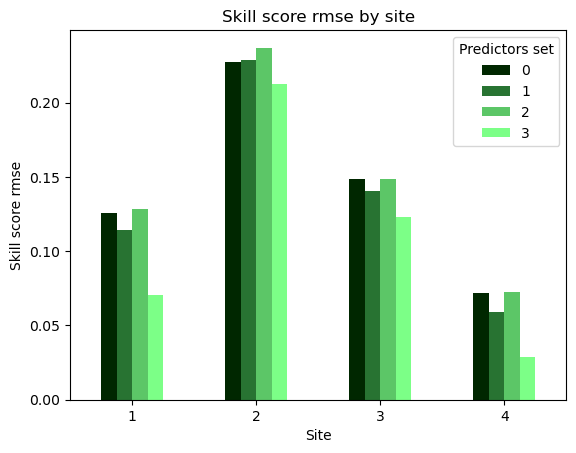
\includegraphics[width=\columnwidth]{figures/first_study/comp_predictors_rmse_mlp.png}
\caption{Comparison of the RMSE skill scores of the different configurations.}
\end{figure}

\begin{figure}[htb!]
    \centering
    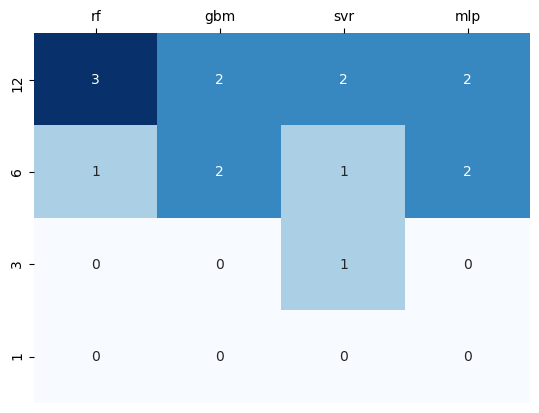
\includegraphics[width=\columnwidth]{figures/first_study/comp_learning_period_rmse.png}
\caption{Pairwise systematicity matrix for RMSE. The value $V_{i,j}$ of the cell $(i,j)$ indicates how often the learning period duration (in months) of line i performs the best, across the 4 sites, for the model of column j. For example, having a 12-months-long learning period is the best thing in 3 sites out of 4 with a SVR model, the last site performs better with a 6-month-long learning period.}
\end{figure}

\begin{figure}[htb!]
    \centering
    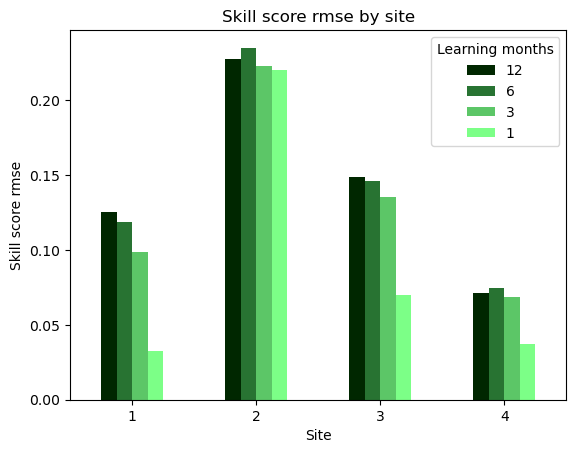
\includegraphics[width=\columnwidth]{figures/first_study/comp_learning_period_rmse_mlp.png}
\caption{Comparison of the RMSE skill scores of the different learning period durations (in months).}
\end{figure}


\begin{figure}[htb!]
    \centering
    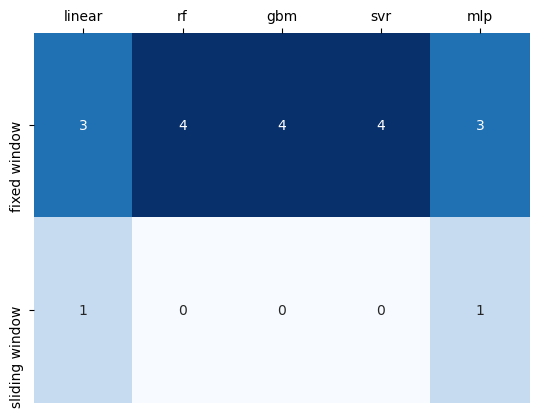
\includegraphics[width=\columnwidth]{figures/first_study/comp_window_rmse.png}
\caption{Pairwise systematicity matrix concerning window type for RMSE.}
\end{figure}

\begin{figure}[htb!]
    \centering
    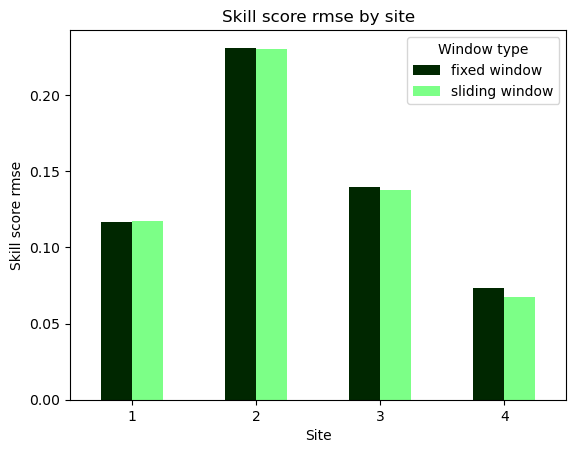
\includegraphics[width=\columnwidth]{figures/first_study/comp_window_rmse_mlp.png}
\caption{Comparison of the RMSE skill scores for a SVR model.}
\end{figure}

\begin{figure}[htb!]
    \centering
    \includesvg[width=\columnwidth]{figures/first_study/comp_for_models_rmse.svg}
\caption{Comparison of the post-processing of four different NWP forecast models on RMSE.}
\end{figure}

\section{Filtering of the measures}